\documentclass{article}
\usepackage[utf8]{inputenc}

\title{Project 2}
\author{Ryan Wood\\
rwood@college.harvard.edu}
\date{May 2018}

\usepackage{tikz}
\usepackage{amsmath}
\usetikzlibrary{arrows}
\usepackage{natbib}
\usepackage{graphicx}
\usepackage{amsmath}
\usepackage{enumerate}
\usepackage[margin=1.4in]{geometry}
\usepackage{fancyhdr}
\usepackage{pgfplots}
\pagestyle{fancy}
\lhead{Dr. Chen}
\chead{Project 2}
\rhead{Ryan Wood}

\begin{document}
\maketitle

\section{Counting Males and Females in the Uncorrected Dataset}
\begin{verbatim}
### list all distinct id numbers
IDs = union(DData$id_num,DData$id_num)
MaleHits = vector(mode = "logical", length = length(IDs))
FemaleHits = vector(mode = "logical", length = length(IDs))

### for each ID, find the corresponding number of male and female hits
for (ii in 1:length(IDs)) {
  visits = subset(DData, id_num == IDs[ii], select=c(gender))
  Ms = 0
  Fs = 0
  for (jj in 1:length(visits[,1])) {
    if (visits$gender[jj] == "M") {
      Ms = Ms + 1
    }
    if (visits$gender[jj] == "F") {
      Fs = Fs + 1
    }
  }
  MaleHits[ii]=Ms;
  FemaleHits[ii]=Fs;
}

### count the number of nonzero male and female hits for each ID
Ms = sum(MaleHits != 0)
Fs = sum(FemaleHits != 0)
\end{verbatim}
The number of unique males was 11459. The number of unique females was 2159, which sums to 13618. The total number of unique people was 13617. We can conclude that there is an error in which someone reported both genders on separate visits to the police office.\\

Now we can count the number of distinct members of each of the following demographics: whites, blacks, asians, hispanics, and other races, of both male and female genders.\\
\begin{verbatim}
### for each ID, find corresponding number of each demographic
MaleHitsB = vector(mode = "logical", length = length(IDs))
FemaleHitsB = vector(mode = "logical", length = length(IDs))
MaleHitsW = vector(mode = "logical", length = length(IDs))
FemaleHitsW = vector(mode = "logical", length = length(IDs))
MaleHitsA = vector(mode = "logical", length = length(IDs))
FemaleHitsA = vector(mode = "logical", length = length(IDs))
MaleHitsH = vector(mode = "logical", length = length(IDs))
FemaleHitsH = vector(mode = "logical", length = length(IDs))
MaleHitsO = vector(mode = "logical", length = length(IDs))
FemaleHitsO = vector(mode = "logical", length = length(IDs))
for (ii in 1:length(IDs)) {
  visits = subset(DData, id_num == IDs[ii], select=c(gender,race))
  MBs = 0
  FBs = 0
  MWs = 0
  FWs = 0
  MAs = 0
  FAs = 0
  MHs = 0
  FHs = 0
  MOs = 0
  FOs = 0
  for (jj in 1:length(visits[,1])) {
    if (visits$gender[jj] == "M" ) {
      if (visits$race[jj] == "B") {
        MBs = MBs + 1
      }
      if (visits$race[jj] == "W") {
        MWs = MWs + 1
      }
      if (visits$race[jj] == "A") {
        MAs = MAs + 1
      }
      if (visits$race[jj] == "H") {
        MHs = MHs + 1
      }
      if (visits$race[jj] == "O") {
        MOs = MOs + 1
      }
    }
    if (visits$gender[jj] == "F") {
      if (visits$race[jj] == "B") {
        FBs = FBs + 1
      }
      if (visits$race[jj] == "W") {
        FWs = FWs + 1
      }
      if (visits$race[jj] == "A") {
        FAs = FAs + 1
      }
      if (visits$race[jj] == "H") {
        FHs = FHs + 1
      }
      if (visits$race[jj] == "O") {
        FOs = FOs + 1
      }
    }
  }
  MaleHitsB[ii]=MBs;
  MaleHitsW[ii]=MWs;
  MaleHitsA[ii]=MAs;
  MaleHitsH[ii]=MHs;
  MaleHitsO[ii]=MOs;
  FemaleHitsB[ii]=FBs;
  FemaleHitsW[ii]=FWs;
  FemaleHitsA[ii]=FAs;
  FemaleHitsH[ii]=FHs;
  FemaleHitsO[ii]=FOs;
}

### count the number of nonzero hits of each demographic for each ID
MBs = sum(MaleHitsB != 0)
FBs = sum(FemaleHitsB != 0)
MWs = sum(MaleHitsW != 0)
FWs = sum(FemaleHitsW != 0)
MAs = sum(MaleHitsA != 0)
FAs = sum(FemaleHitsA != 0)
MHs = sum(MaleHitsH != 0)
FHs = sum(FemaleHitsH != 0)
MOs = sum(MaleHitsO != 0)
FOs = sum(FemaleHitsO != 0)
\end{verbatim}

The output is:\\

\begin{tabular}{l*{6} c r}
       & Black & White & Asian & Hispanic & Other & Total \\
Male   & 8838 & 2070 & 49 & 517 & 15 & 11489 \\
Female & 1494 & 634 & 6 & 30 & 5 & 2169 \\
Total  & 10332 & 2704 & 55 & 547 & 20 & 13658 \\
\end{tabular}\\

The total of 13658 is 41 more than the number of distinct visitors (13617). From this we can conclude that some visitors must have reported different ethnicities on their separate visits.\\

\section{Counting Males and Females in the Corrected Dataset}
We use the same code as in the previous section, but with the corrected dataset. The number of distinct males was 11458. The number of distinct females is 2159. This sums to 13617, which is the same as the number of distinct visitors.\\

Now we can consider the number of distinct members of each of the following demographics: whites, blacks, asians, hispanics, and other races, of both male and female genders.\\

\begin{tabular}{l*{6} c r}
       & Black & White & Asian & Hispanic & Other & Total \\
Male   & 8829 & 2056 & 47 & 507 & 19 & 11458 \\
Female & 1491 & 628 & 4 & 28 & 8 & 2159 \\
Total  & 10320 & 2684 & 51 & 535 & 27 & 13617 \\
\end{tabular}\\

\section{Additional Questions for the Cleaned Data}
The number of visitors with 1,2,3,4, and 5+ additional images.\\
\begin{verbatim}
### find the number of males and females with 1,2,3,4,5+ extra visits
M1 = sum(MaleHits == 2)
M2 = sum(MaleHits == 3)
M3 = sum(MaleHits == 4)
M4 = sum(MaleHits == 5)
M5 = sum(MaleHits > 5)

F1 = sum(FemaleHits == 2)
F2 = sum(FemaleHits == 3)
F3 = sum(FemaleHits == 4)
F4 = sum(FemaleHits == 5)
F5 = sum(FemaleHits > 5)
\end{verbatim}
\begin{tabular}{l*{6} c r}
       & 1 & 2 & 3 & 4 & 5+ & Total \\
Male   & 2350 & 3606 & 1975 & 1135 & 2020 & 11086 \\
Female & 478 & 712 & 352 & 172 & 360 & 2074 \\
Total  & 2828 & 4318 & 2327 & 1307 & 2380 & 13160 \\
\end{tabular}\\\\


The number of visitors at each decade of life at time of first visit:\\

\begin{verbatim}
### find number of males and females with first-visit ages in the ranges
AgeM1 = sum(MaleHitsAge < 20)
AgeM2 = sum(MaleHitsAge >= 20 & MaleHitsAge < 30)
AgeM3 = sum(MaleHitsAge >= 30 & MaleHitsAge < 40)
AgeM4 = sum(MaleHitsAge >= 40 & MaleHitsAge < 50)
AgeM5 = sum(MaleHitsAge >= 50 & MaleHitsAge < 999)

AgeF1 = sum(FemaleHitsAge < 20)
AgeF2 = sum(FemaleHitsAge >= 20 & FemaleHitsAge < 30)
AgeF3 = sum(FemaleHitsAge >= 30 & FemaleHitsAge < 40)
AgeF4 = sum(FemaleHitsAge >= 40 & FemaleHitsAge < 50)
AgeF5 = sum(FemaleHitsAge >= 50 & FemaleHitsAge < 999)
\end{verbatim}

\begin{tabular}{l*{6} c r}
       & $\leq19$ & 20-29 & 30-39 & 40-49 & 50+ & Total \\
Male   & 1968 & 3387 & 3047 & 2302 & 754 & 11458 \\
Female & 294 & 607 & 686 & 473 & 99 & 2159 \\
Total  & 2262 & 3994 & 3733 & 2775 & 853 & 13617 \\
\end{tabular}\\

\section{BIF Data by Race}
\begin{verbatim}
rm(list=ls())
BIFData = read.csv("/Users/ryanwood/Documents/Summer 2018 - UNCW /Project 1-May 22, 2018/MorphII_BIF_s7-37_g0.1_max_partial.csv",header = F);
CData = read.csv("/Users/ryanwood/Documents/Summer 2018 - UNCW /Project 2-May 23, 2018/morphII_clean.csv",header=TRUE);
indexes = rep(0,length(BIFData[,1]))

### make a vector with the indexes of each of the rows in BIFData
for (ii in 1:length(indexes)) {
  tmpInfo = as.character(BIFData[ii,1])
  tmpInfo = substr(tmpInfo,1,6)
  indexes[ii] = tmpInfo
}

### replace the first column of BIFData with the race of the corresponding
BIFData$V1 = as.character(BIFData$V1)
for (ii in 1:length(indexes)) {
  curPerson = subset(CData,id_num == as.numeric(indexes[ii]))
  race = as.character(curPerson$race[1])
  BIFData$V1[ii] = race
}

### run summary statistics on the male and female subsets of BIFData
BBIF = filter(BIFData,V1=="B")
WBIF = filter(BIFData,V1=="W")
ABIF = filter(BIFData,V1=="A")
HBIF = filter(BIFData,V1=="H")
OBIF = filter(BIFData,V1=="O")

len = length(BBIF[1,])
boxplot(as.numeric(unlist(BBIF[,2:len])),as.numeric(unlist(WBIF[,2:len])),as.numeric(unlist(ABIF[,2:len])),as.numeric(unlist(HBIF[,2:len])),as.numeric(unlist(OBIF[,2:len])),main="BIFs - Black, White, Asian, Hispanic, Other")
\end{verbatim}

Now we look at some graphical and numerical summaries for the BIF data by race.\\

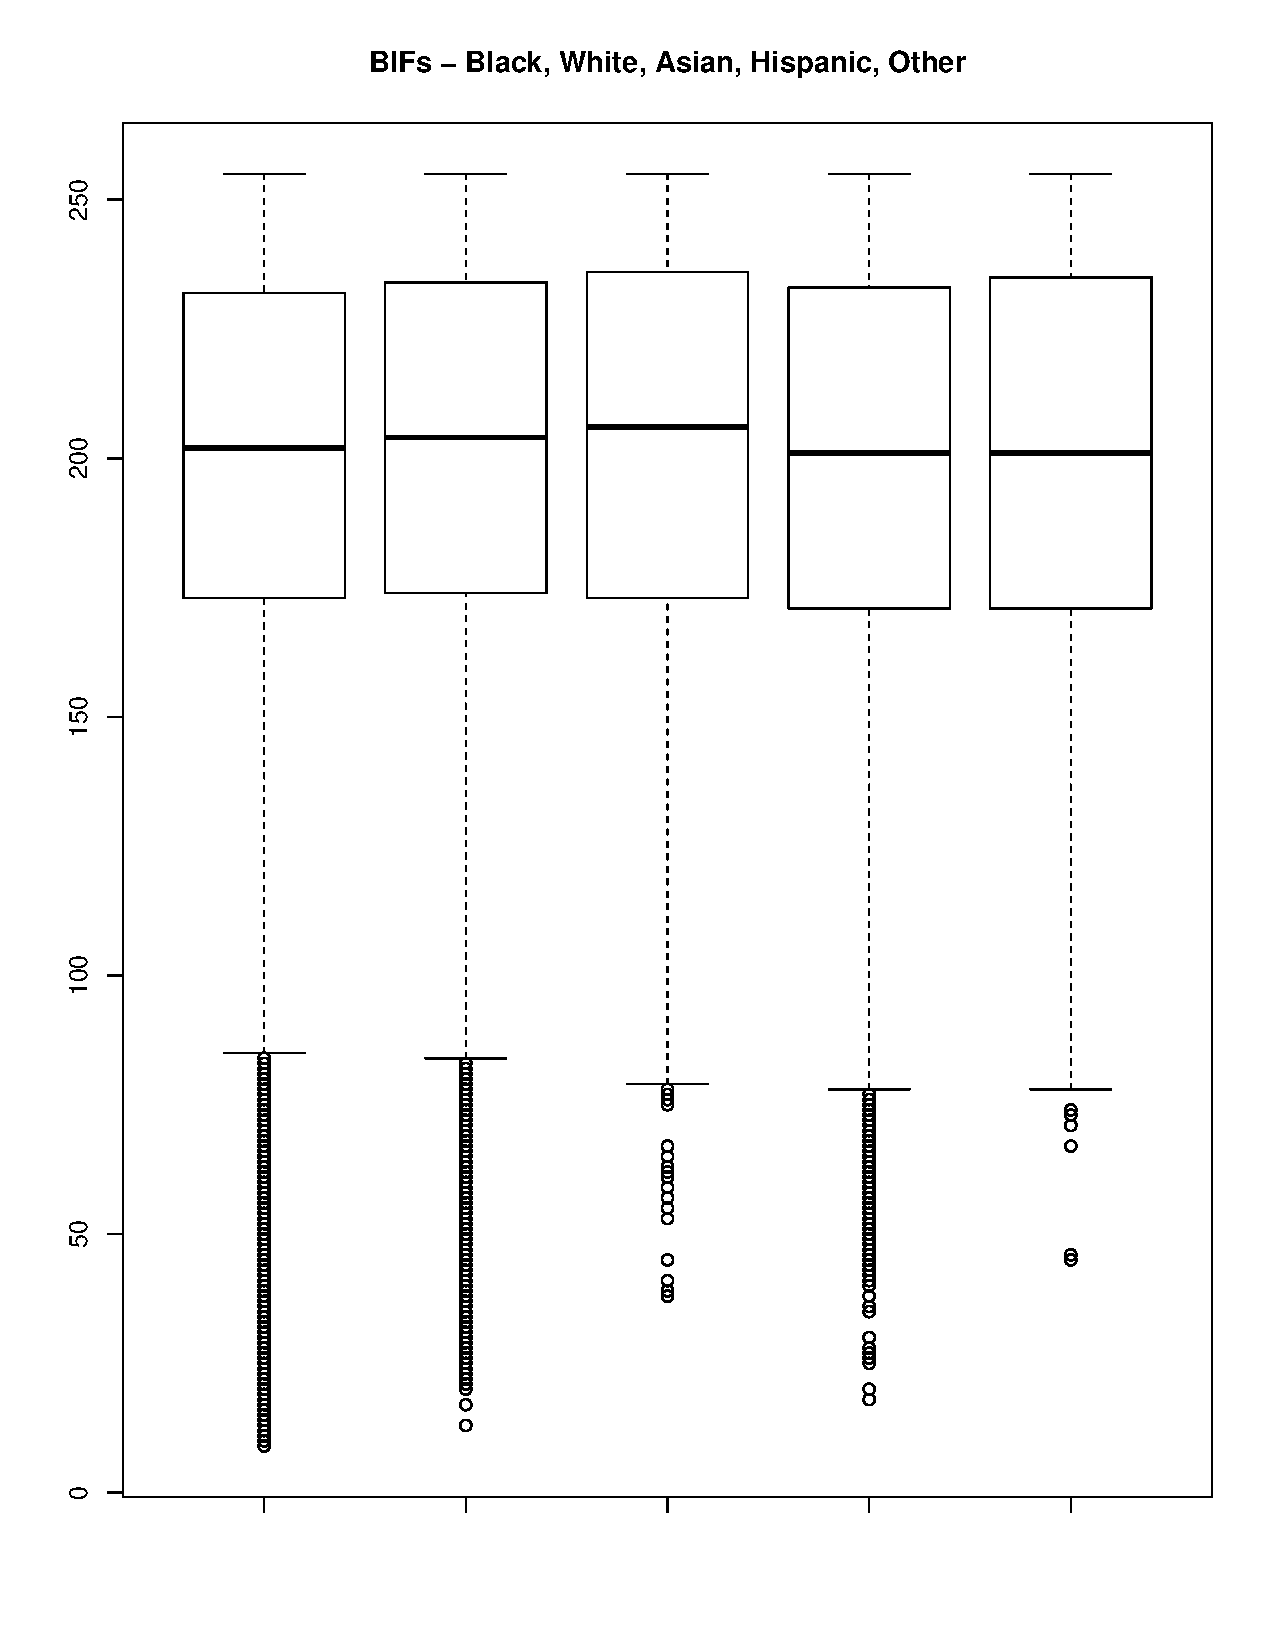
\includegraphics[width=0.5\textwidth]{PART4.pdf}

\end{document}
